%%%%%%%%%%%%%%%%%%%%%%%%%%%%%%%%%%%%%%%%%
% Journal Article
% LaTeX Template
% Version 1.4 (15/5/16)
%
% This template has been downloaded from:
% http://www.LaTeXTemplates.com
%
% Original author:
% Frits Wenneker (http://www.howtotex.com) with extensive modifications by
% Vel (vel@LaTeXTemplates.com)
%
% License:
% CC BY-NC-SA 3.0 (http://creativecommons.org/licenses/by-nc-sa/3.0/)
%
%%%%%%%%%%%%%%%%%%%%%%%%%%%%%%%%%%%%%%%%%

%----------------------------------------------------------------------------------------
%	PACKAGES AND OTHER DOCUMENT CONFIGURATIONS
%----------------------------------------------------------------------------------------

%\documentclass[10pt]{article} % Single column

\documentclass[colorinlistoftodos,twoside,twocolumn]{article} % Two column

\usepackage{blindtext} % Package to generate dummy text throughout this template 

\usepackage[sc]{mathpazo} % Use the Palatino font
\usepackage[T1]{fontenc} % Use 8-bit encoding that has 256 glyphs
\linespread{1.05} % Line spacing - Palatino needs more space between lines
\usepackage{microtype} % Slightly tweak font spacing for aesthetics

\usepackage[spanish]{babel} % Language hyphenation and typographical rules

\usepackage[hmarginratio=1:1,top=32mm,columnsep=20pt]{geometry} % Document margins
\usepackage[hang, small,labelfont=bf,up,textfont=it,up]{caption} % Custom captions under/above floats in tables or figures
\usepackage{booktabs} % Horizontal rules in tables

\usepackage{lettrine} % The lettrine is the first enlarged letter at the beginning of the text

\usepackage{enumitem} % Customized lists
\setlist[itemize]{noitemsep} % Make itemize lists more compact

\usepackage{abstract} % Allows abstract customization
\renewcommand{\abstractnamefont}{\normalfont\bfseries} % Set the "Abstract" text to bold
\renewcommand{\abstracttextfont}{\normalfont\small\itshape} % Set the abstract itself to small italic text

\usepackage{titlesec} % Allows customization of titles
\renewcommand\thesection{\Roman{section}} % Roman numerals for the sections
\renewcommand\thesubsection{\roman{subsection}} % roman numerals for subsections
\titleformat{\section}[block]{\large\scshape\centering}{\thesection.}{1em}{} % Change the look of the section titles
\titleformat{\subsection}[block]{\large}{\thesubsection.}{1em}{} % Change the look of the section titles

\usepackage{fancyhdr} % Headers and footers
\pagestyle{fancy} % All pages have headers and footers
\fancyhead{} % Blank out the default header
\fancyfoot{} % Blank out the default footer
\fancyhead[C]{Music Genre Classifier} % Custom header text
\fancyfoot[RO,LE]{\thepage} % Custom footer text

\usepackage{titling} % Customizing the title section

\usepackage[colorlinks]{hyperref} % For hyperlinks in the PDF

\usepackage{graphicx} % For images
\usepackage{subcaption}

\usepackage{pifont} % bullets

\usepackage{amsmath}


% Keywords command
\providecommand{\keywords}[1]
{
	\small	
	\vspace{0.5em}
	\noindent \textbf{\textit{Palabras clave --- }} #1
}

%----------------------------------------------------------------------------------------
%	TITLE SECTION
%----------------------------------------------------------------------------------------

\setlength{\droptitle}{-4\baselineskip} % Move the title up

\pretitle{\begin{center}\Huge\bfseries} % Article title formatting
	\posttitle{\end{center}} % Article title closing formatting
\title{\normalsize{Proyecto Final de Aprendizaje de Máquina}\\
	\Huge\bfseries Music Genre Classifier\\
} % Article title
\author{% 
	\normalsize\textsc{Integrantes:}\\
	\normalsize\textsc{Leandro Rodr\'iquez Llosa  C-41X}\\[2ex]
	\normalsize\textsc{Niley Gonz\'alez Ferrales.  C-411}\\[2ex]
	\normalsize\textsc{Arian Pazo Valido.  C-311} \\[2ex]
	%\normalsize\textsc{Grupo: C-41X} \\[2ex]
	\small Cuarto a\~no. Ciencias de la Computaci\'on. \\ % institution
	\small Facultad de Matem\'atica y Computaci\'on, Universidad de La Habana, Cuba \\ % institution
}
\date{\footnotesize Junio 2023 } % Leave empty to omit a date


% Abstract configurations
\renewenvironment{abstract}
{\small
	\begin{center}
		\bfseries \abstractname\vspace{-.5em}\vspace{0pt}
	\end{center}
	\list{}{
		\setlength{\leftmargin}{0.9cm}%
		\setlength{\rightmargin}{\leftmargin}%
	}%
	\item\relax}
{\endlist}


\usepackage{todonotes} % \TODO
\usepackage{listings} % Code listings
\usepackage{xcolor}
\definecolor{backcolour}{rgb}{0.95,0.95,0.92}

\newcommand{\csl}[1]{\colorbox{backcolour}{\texttt{#1}}}

\newcommand{\imgcaption}[2]{\tiny \textbf{Figura #1.} #2.}

\newcommand{\mgc}[2][]{\colorbox{backcolour}{\texttt{\_\_#2\_\_#1}}}

\newcommand{\mgccapt}[1]{\texttt{\_\_#1\_\_}}

% Hyperlinks configurations
\hypersetup{
	colorlinks=true,
	linkcolor=black,
	filecolor=magenta,      
	urlcolor=cyan,
	pdftitle={Overleaf Example},
	pdfpagemode=FullScreen,
}

%----------------------------------------------------------------------------------------

\begin{document}
	% Print the title
	\maketitle

    \selectlanguage{spanish}
	\pagenumbering{gobble}
	\begin{abstract}

		\todo{TODO}

		\vspace{1em}
		\keywords{ 
			aprendizaje automático \textbf{$\cdot$} clasificación \textbf{$\cdot$}  géneros musicales \textbf{$\cdot$} transformada wavelet discreta \textbf{$\cdot$} transformada wavelet compleja de doble árbol
		}

	\end{abstract}
	
	%----------------------------------------------------------------------------------------
	%	ARTICLE CONTENTS
	%----------------------------------------------------------------------------------------
	
	\section{Introducción}
	
    \todo{TODO}
	 La clasificación de géneros basada en la Transformada de Fourier, utilizando MFCC y espectrogramas, se ha explorado con éxito en los últimos años. Aunque la Transformada de Fourier tiene una alta resolución en el dominio de la frecuencia, tiene una resolución cero en el dominio del tiempo. Esto significa que puede decirnos exactamente qué frecuencias están presentes en una señal, pero no en qué lugar en el tiempo se han producido \cite{wavelet transform in machine learning}. Un mejor enfoque para analizar señales con un espectro de frecuencias dinámico es la Transformada Wavelet. Esta tiene una alta resolución tanto en el dominio de la frecuencia como en el del tiempo. Además, la Transformada Wavelet puede proporcionar una resolución de frecuencia variable, lo que significa que puede adaptarse a diferentes escalas de tiempo y frecuencia. Esto puede ser útil en la clasificación de géneros musicales, donde ciertos géneros pueden tener patrones rítmicos más rápidos o lentos que otros \cite{Musical Genre Classification Of Audio Signals}. Por último, la Transformada Wavelet, ya que utiliza pocos datos para representar una señal puede ser útil en la clasificación de géneros musicales; donde el procesamiento de grandes cantidades de datos suele ser costoso en términos de tiempo y recursos computacionales.   

	\section{Propuesta}
	
	
	
Hasta ahora hemos implementado algunas de las ideas m\'as exitosas para clasificar g\'eneros musicales que se pueden encontrar en el estado del arte. Pero resulta que ninguna de estas hace uso de la letra de la canci\'on, la cu\'al sabemos intuitivamente que puede aportar bastante informaci\'on sobre el g\'enero de la canci\'on. Por tanto, una idea implementada en este trabajo es hacer un modelo clasificador que conste de una red neuronal que combina análisis de la letra, mediante un embedding que represente a la misma, y de la música con un encoder. La idea de este modelo es concatenar los vectores resultantes de estos procesamientos y clasificar en base a esta combinación de features. 
	
	\subsection{Autoencoder}
Para construir el encoder se programó un autoencoder y se tomó el modelo hasta el bottleneck para sacar el encoder. La arquitectura del autoencoder combinó capas maxpooling y upsampling al inicio y al final respectivamente para moderar el tamaño la imagen, intercaladas con capas convolucionales y en el medio tuvo un par de capas densas para aprovechar que ya el número de dimensiones era relativamente pequeño y realizar un poco más de aprendizaje. La arquitectura en detalle es la siguente:
\begin{center}
  \begin{tabular}{ | c | c | c |}
    \hline
    \textbf{Nombre de la capa} & \textbf{Tipo de la capa} & \textbf{Shape de salida} \\ \hline
    $input_l$ & Input & (192, 256, 3) \\ \hline
    $maxp_{ini}$ & MaxPooling2D & (96, 128, 3) \\ \hline
    $encoding_1$ & Conv2D & (96, 128, 12) \\ \hline
    $maxp_1$ & MaxPooling2D & (48, 64, 12) \\ \hline
    $encoding_2$ & Conv2D & (48, 64, 6) \\ \hline
    $maxp_2$ & MaxPooling2D & (24, 32, 6) \\ \hline
    $encoding_3$ & Conv2D & (24, 32, 3) \\ \hline
    $flat_1$ & Flatten & (2304) \\ \hline
    $bottleneck$ & Dense & (500) \\ \hline
    $decoding_1$ & Dense & (2304) \\ \hline
    $resh_1$ & Reshape & (24, 32, 3) \\ \hline
    $decoding_2$ & Conv2D & (24, 32, 6) \\ \hline
    $Up_1$ & UpSampling2D & (48, 64, 6) \\ \hline
    $decoding_3$ & Conv2D & (48, 64, 12) \\ \hline
    $Up_2$ & UpSampling2D & (96, 128, 12) \\ \hline
    $decoding_4$ & Conv2D & (96, 128, 3) \\ \hline
    $output_l$ & UpSampling2D & (192, 256, 3) \\
    \hline
  \end{tabular}
\end{center}

Como se puede observar la arquitectura es casi simétrica.

Se tomó como función de pérdida y métrica el error cuadrático medio ($\textit{mean squared error}$). La entrada del autoencoder y la salida esperada fueron las imágenes del feature MFCC del conjunto de entrenamiento luego de haber sido normalizadas, es decir, que en vez de estar en el rango $[0, 255]$ cada valor de la imagen de entrada, los representamos en el rango $[0, 1]$. 

Anteriormente se probaron otras arquitecturas, desde algunas que no tenían capas densas hasta otras que principalmente consistían en capas densas. El problema en las arquitecturas carentes de capas densas era que sus resultados no eran lo suficientemente buenos, es decir, debido a su relativamente baja cantidad de parámetros el nivel de aprendizaje que podían lograr era inferior al que se logró luego con arquitecturas con capas densas. Por otro lado, las arquitecturas que consistían principalmente en capas densas tenían problemas como que los modelos eran muy grandes, algunos pasando de los GiB de almacenamiento y presentaban un problema para nosotros a la hora del entrenamiento. Otro problema que tienen las arquitecturas más basadas en capas densas es su tendencia al overfitting. En las prueba realizadas, las arquitecturas carentes de capas densas no presentaban este tipo de problema ya que los resultados en los conjuntos de entrenamiento, test y validación tenían poca diferencia entre ellos, sin embargo en las arquitecturas que tenían capas densas, por el gran número de parámetros si se evidencia una diferencia sustancial entre los resultados en los conjuntos de entrenamiento, y los obtenidos en los de prueba y validación. Al entrenar se realizó un $save$ cada $10$ epochs. Veamos los resultados sobre el número del $save$ en el modelo de autoencoder presentado:
\begin{figure}[h!]
  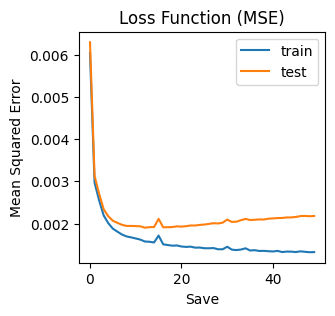
\includegraphics[width=\linewidth]{overfitting_graph.png}
\end{figure}

A partir del análisis de la gráfica anterior se tomó como cantidad de epochs a ejecutar la cantidad de $150$, ya que se conjeturó (y luego validó) que el comportamiento del modelo en el conjunto de prueba sería muy similar al comportamiento en el conjunto de validación y en este punto es que se obtiene un mejor performance en el conjunto de prueba. 

Volviendo atrás, los resultados obtenidos para cada tipo de modelo:
\begin{itemize}
	\item los modelos que no tenían capas densas lograron primeramente un error (MSE) de $0.0025$ y luego de ampliar la   cantidad de dimensiones que salen del bottleneck, es decir la cantidad de dimensiones de la representación se logró $0.0021$. Estos modelos tenían muy poco overfitting luego de $500$ epochs.
	\item los modelos que presentan capas densas, por su parte, comenzaron con resultados en el conjunto de entrenamiento de hasta $0.0011$ con $500$ epochs, lo cual era muy bueno pero podía implicar overfitting. A medida que se redujeron la cantidad de parámetros (de $288$ millones a los $2.3$ millones del modelo propuesto) los resultados en el conjunto de entrenamiento fueron peores pero nunca sobrepasaron el valor de $0.0013$ en $500$ epochs. Luego de correr el modelo propuesto solo $150$ epochs se obtuvieron los mejores resultados tanto en el conjunto de prueba como en el validación, oscilando alrededor de $0.00185$, por su lado en el conjunto de entrenamiento se obtuvieron resultados alrededor de $0.0016$, lo que evidencia la presencia de overfitting.
\end{itemize}

\subsection{Feature: Letra de la canci\'on}

La segunda mitad de la informaci\'on de la que queremos que nuestro modelo aprenda es la letra de la canci\'on. Para ello lo primero que se hace es extraer la misma haciendo uso del conocido modelo de Whisper (ver \cite{whisper}). Luego necesitamos un embedding que represente al texto de la canci\'on que vamos a necesitar para entrenar y evaluar el modelo. Para extraer el mismo hacemos uso de otro modelo de aprendizaje de m\'aquinas conocido como Bert (ver \cite{bert}). Este \'ultimo es un modelo basado en redes neuronales para el procesamiento de lenguaje natural, desarrollado por Google.

\subsection{Arquitectura del modelo}

Una vez obtenidos los dos embedding correspondientes a la letra de la canci\'on y la m\'usica (MFCC) ya tenemos la capa de entrada de nuestra red neuronal. La misma es la concatenaci\'on de los dos vectores obtenidos. Luego la red tiene  dos capas ocultas con funci\'on de activaci\'on RELU y cantidad de neuronas $128$ y $64$ respectivamente. Finalmente la capa de salida consiste de $10$ neuronas que representan a cada uno de los g\'eneros musicales que analizamos, y cuenta con softmax como funci\'on de activaci\'on. Siendo coherente con esto \'ultimo usamos como funci\'on de p\'erdida la Categorical Cross Entropy. Adem\'as, el modelo fue entrenado durante $500$ epochs.


\subsection{Resultados}

Como podemos ver en la siguiente gr\'afica el valor de ``accuracy'' de nuestro modelo para el training set es casi perfecto llegados al epoch n\'umero $300$. En el caso del conjunto de  datos de validaci\'on, que es el que nos da la efectividad de nuestro modelo, vemos que el accuracy crece r\'apidamente hasta llegar al valor $0.57$ alrededor del epoch $150$.

 \begin{figure}[h!]
 	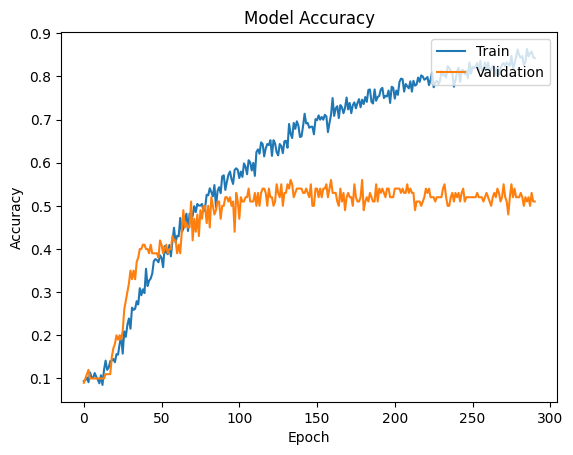
\includegraphics[width=\linewidth]{vl_accuracy.png}
 \end{figure}

Con m\'as capas y neuronas en nuestro modelo, este hac\'ia r\'apidamente overfitting, o sea en pocos epochs. Esto nos llev\'o a reducirlo a la arquitectura actual. Como podemos observar en la pr\'oxima gr\'afica la funci\'on de p\'erdida para los datos entrenantes decrece r\'apidamente acerc\'andose mucho a cero en el epoch $300$. En el caso de los datos de validaci\'on, vemos como a partir del epoch $100$ la red comienza a hacer overfitting, pero no es representativo. 

 \begin{figure}[h!]
	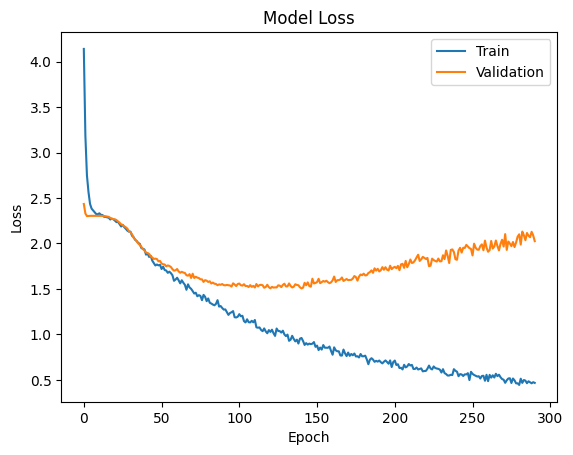
\includegraphics[width=\linewidth]{vl_loss.png}
\end{figure}

%Presentamos aqu\'i adem\'as la matriz de confusi\'on.

 \begin{figure}[h!]
	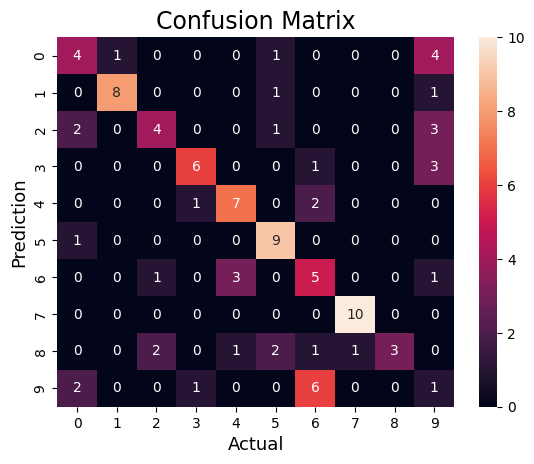
\includegraphics[width=\linewidth]{vl_confussion_matrix.png}
\end{figure}

Finalmente con un accuracy de $0.57$ y con valor para la funci\'on de p\'erdida de  $2.9323$ llegamos a la conclusi\'on de que este modelo no arroja resultados que mejoren los obtenidos en los modelos ya vistos antes.

Se realizó también cross validation con Kfold dividiendo todo el conjunto de entrenamiento en $10$ subconjuntos. Los resultados del cross validation coincidieron con los resultados anteriormente descrito. Este test se hizo luego de haber fijado la cantidad de epochs en $150$.
	\subsection{Wavelets}
	Proponemos dos métodos de extracción de características usando varias formas de Transformadas Wavelet. 
    El primero es la Transformada Wavelet Discreta (DWT) \cite{wavelet transform in machine learning} y el segundo la Transformada Wavelet Compleja de Doble Árbol (DT-CWT) \cite{DT-CWT}.
    
    La DWT es un caso especial de Transformada Wavelet que proporciona una representación compacta de la señal en el tiempo y la frecuencia que se puede calcular de manera eficiente\cite{Musical Genre Classification Of Audio Signals}. La DT-CWT es una mejora relativamente reciente a DWT; ya que para señales moduladas complejas como el audio, DWT encuentra algunas pocas deficiencias: oscilaciones, varianza de desplazamiento, aliasing y falta de direccionalidad\cite{Wavelet Transform for Music Genre Classification}. 
    
    El pipeline para ambos métodos consiste en calcular las respectivas características para cada canción del dataset. Luego con la matriz obtenida se realiza un split de $80\%$ - $20\%$ y se entrena el modelo de machine learning elegido. Ajustando los hiperparámetros utilizando Cross-Validation.
    \todo{TODO}

	\section{Tests}

    \todo{TODO}
    	Para la implementación utilizando Transformadas Wavelet fueron probados varios modelos de machine learning tradicional como Logistic Regression, SVC, Linear SVC, Random Forest Classifier y Gradient Boosting Classifier. Como los dos últimos se comportan mejor en aproximadamente más de 10\% de precisión respecto al resto, decidimos enfocarnos en esos modelos . 
    
    Respecto a la Transformada Wavelet Discreta, Daubechies wavelet  empíricamente, muestra el mejor comportamiento en muchas aplicaciones\cite{Wavelet Transform for Music Genre Classification}. Experimentamos con distintos órdenes de Daubechies wavelet, y db12 mostró el mejor comportamiento. Los mejores resultados para DWT fueron obtenidos con Random Forest; utilizando como parámetros: \emph{n\_estimators=100}, \emph{max\_depth=13}, \emph{bootstrap=False}. La precisión con este modelo se ubicaba alrededor de $0.77$. \\

% \usepackage{subcaption}
\begin{figure} % Start the main figure environment
    \centering
    \begin{subfigure}{0.45\linewidth} % First subfloat environment

        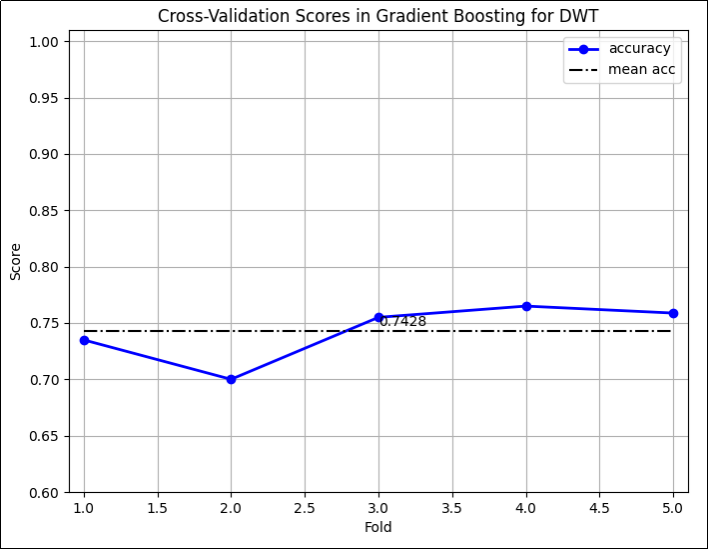
\includegraphics[width=.95\linewidth]{images/CV_DWT_gb.png}         \caption{DWT Gradient Boosting}
    \end{subfigure}
    \hskip 1em plus 1fill minus 1fil
    \begin{subfigure}{0.45\linewidth} % Second subfloat environment
        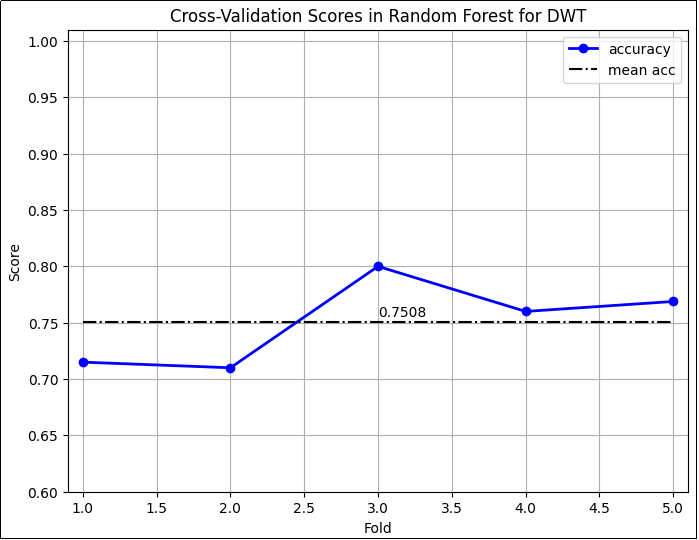
\includegraphics[width=.95\linewidth]{images/CV_DWT_rf.png}         \caption{DWT Random Forest}
    \end{subfigure}
    \caption{ DWT Cross-Validation}
\end{figure}

  La Transformada Wavelet Compleja de Doble Árbol, mostró los mejores resultados con 17 niveles de descomposición para extraer los coeficientes wavelet. Se comporta mejor que DWT, alcanzando más de $0.8$ de precisión con Random Forest Classifier.  Además de las imagenes del Cross-Vlidation también reportamos una matriz de confusión para comprobar el comportamiento en cada género. Se observa que no se desempeña de la misma forma en todos los géneros, ya que hay algunos (como el metal o el jazz) donde se observan muy buenos resultados. \\

\begin{figure} % Start the main figure environment
    \centering
    \begin{subfigure}{0.45\linewidth} % First subfloat environment

        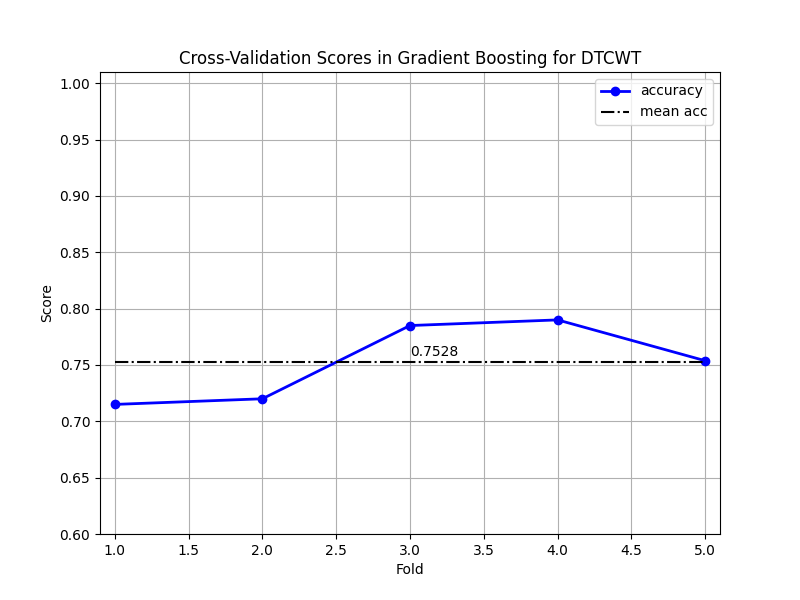
\includegraphics[width=.95\linewidth]{images/CV_DTCWT_gb.png}         \caption{DTCWT Gradient Boosting}
    \end{subfigure}
    \hskip 1em plus 1fill minus 1fil
    \begin{subfigure}{0.45\linewidth} % Second subfloat environment
        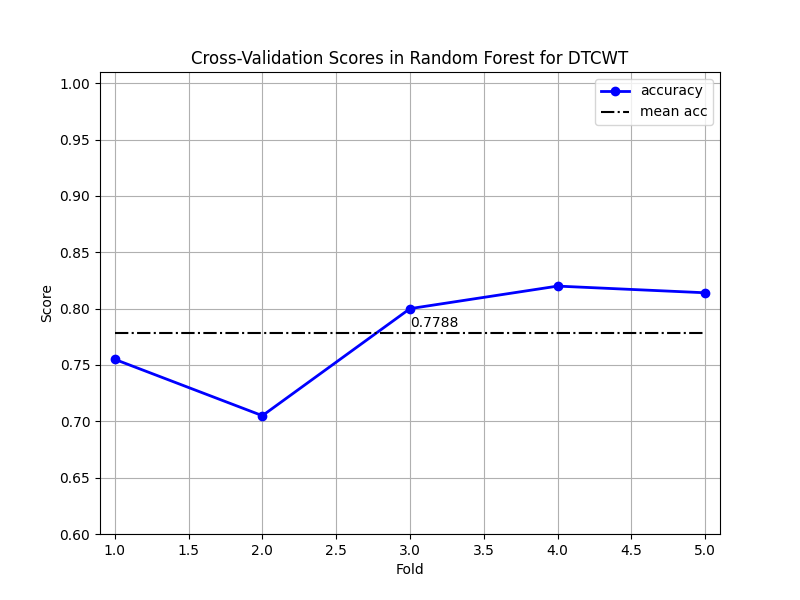
\includegraphics[width=.95\linewidth]{images/CV_DTCWT_rf.png}         \caption{DTCWT Random Forest}
    \end{subfigure}
    \caption{DTCWT Cross-Validation}
\end{figure}

\begin{figure} 
    \centering    
    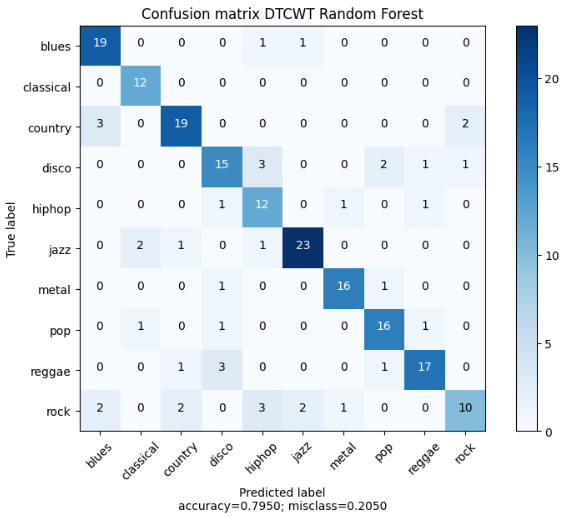
\includegraphics[width=.8\linewidth]{images/conf_matrix_DTCWT.png}    
    \caption{DTCWT Random Forest Matriz de Confusi\'on}
\end{figure}

	\section{Recomendaciones}
	
    \todo{TODO}
    
\begin{thebibliography}{20}
	\bibitem{whisper} A. Radford, J. Wook Kim, T. Xu, G. Brockman, C. McLeavey y I. Sutskever: \emph{RobustSpeechRecognitionviaLarge-ScaleWeakSupervision}. Preprint on arXiv: 2212.04356, 2022. 
	
		\bibitem{bert} J. Devlin, M. Chang, K. Lee y K. Toutanova: \emph{BERT:Pre-trainingofDeepBidirectionalTransformersfor LanguageUnderstanding}. Preprint on arXiv: 1810.04805, 2018. 
	
	\bibitem{murphy} Kevin P. Murphy: \emph{Machine Learning: A Probabilistic Perspective}. MIT Press, 2012.
	\bibitem{Wavelet Transform for Music Genre Classification} Pranav Vijaya Kumar Rao, Vishwas Nagesh Moolimani: \emph{ECG Analysis based feature extraction using Wavelet Transform for Music Genre Classification}, 2020. 
	\bibitem{wavelet transform in machine learning} Ahmet Taspinar: \emph{A guide for using the wavelet transform in machine learning}, unpublished. [Online]. Available: http://ataspinar.com/2018/12/21/a-guide-for-using-the-wavelet-transform-in-machine-learning/
	\bibitem{DT-CWT} Selesnick, I.W. and Baraniuk, R.G. and Kingsbury, N.C., \emph{The dual-tree complex wavelet transform}, 2005, IEEE Signal Processing Magazine, pp. 123-151.
	\bibitem{Wavelets y sus Aplicaciones} Liliana R. Castro, Silvia M.  Castro: \emph{Wavelets y sus Aplicaciones}, ler. Congreso Argentino de Ciencias de la Computación, pp. 195-204.
	\bibitem{Musical Genre Classification Of Audio Signals} George Tzanetakis, Georg Essl, Perry Cook: \emph{Automatic Musical Genre Classification Of Audio Signals}
    \todo{TODO}
	
\end{thebibliography}
\end{document}

